
\textbf{Notation}
\begin{itemize}
	\item number of features: $n_x$
	\item $(x, y)$
	\item $x \in \mathbb{R}^{n_x}$
	\item $m$ training samples: $(x^{(1)}, y^{(1)}), \dots, (x^{(m)}, y^{(m)})$
	\item $X = \begin{bmatrix}
	\vline & & \vline \\
	x^{(1)} & \dots & x^{(m)}\\ 
	\vline & & \vline \\
	\end{bmatrix}$, EACH ROW IS A FEATURE. $X_{n_x \times m}$. This way, implementation will be much easier. 
	\item $Y = \begin{bmatrix}
	y^{(1)}, \dots, y^{(m)}
	\end{bmatrix}$, $Y_{1\times m}$
\end{itemize}

\subsection{Logistic Regression}
Given $X$, want $\yhat = P(y=1|X)$, knowing that $x_i \in \mathbb{R}^{n_x}$. 

Parameters: $w \in \mathbb{R}^{n_x}$, $b \in \mathbb{R}$

Output: $\sigma(w^Tx + b)$, given that $\sigma(z) = \frac{1}{1+e^{-z}}$

Loss function: $L(\yhat, y) = -\Big(ylog(\yhat) + (1-y)log(1-\yhat)\Big)$
\begin{itemize}
	\item if $y = 1$, $Loss = - log(\yhat)$, so we want $\log(\yhat)$ and therefore $\yhat$ as big as possible (one) to minimize the loss. 
	\item if $y = 0$, $Loss = - log(1-\yhat)$, so we want $\log(1-\yhat)$ and therefore $1-\yhat$ as big as possible, which means $\yhat$ as small as possible (zero)), to minimize the loss. 

	\item Cost function: 
$$
J(w, b) = \frac{1}{m} \sum_{i = 1}^{m} L(y^{(i)}, y) = \frac{-1}{m} \sum_{i = 1}^{m} \Big[ylog(\yhat^{(i)}) + (1-y)log(1-\yhat^{(i)})\Big]
$$
\end{itemize}

\subsection{Gradient Descent}
We want to find $w, b$ such that $J(w, b)$ is minimized. 
\begin{itemize}
	\item Repeat:
	\begin{itemize}
		\item[] $w = w - \alpha \frac{\partial J(w, b)}{\partial w}$
		\item[] $b = b - \alpha \frac{\partial J(w, b)}{\partial b}$
	\end{itemize}
\end{itemize}

\subsection{Partial Derivatives}
\begin{figure}[h]
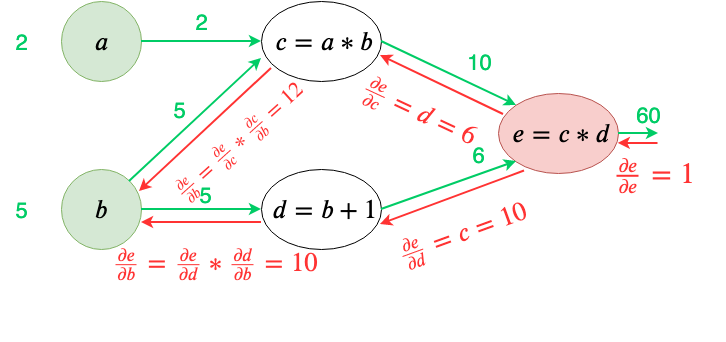
\includegraphics[width=8cm]{images/partial.png}
\centering
\end{figure}

\subsection{Gradient Descent for Logistic Regression}
Feed Forward: 
$$
z = w^Tx + b
$$
$$
\yhat = a = \sigma(z)
$$
$$
x = \begin{bmatrix}
x_1\\
x_2
\end{bmatrix}, 
w = \begin{bmatrix}
w_1\\
w_2
\end{bmatrix}
$$
$$
z = w_1x_1 + w_2x_2 + b
$$
$$
a = \sigma(z), L(a, y) = -\Big(ylog(a) + (1-y)log(1-a)\Big)
$$
Notation: 
$$
dx = \frac{dL}{dx}
$$
Now backpropagate: 
$$
da = \frac{dL}{da} = -\frac{y}{a} + \frac{1-y}{1-a}
$$
$$
dz = \frac{dL}{dz} = \frac{dL}{da}\frac{da}{dz} = \Big[-\frac{y}{a} + \frac{1-y}{1-a}\Big]\Big[a(1-a)\Big] = a - y
$$
$$
dw_1 = \frac{dL}{dw_1} = \frac{dL}{dz}\frac{dz}{dw_1} = x_1 dz
$$
$$
dw_2 = \frac{dL}{dw_2} = \frac{dL}{dz}\frac{dz}{dw_2} = x_2 dz
$$
$$
db = \frac{dL}{db} = \frac{dL}{dz}\frac{dz}{db} = dz
$$
%\newpage
\subsection{Gradient Descent on $m$ Training Samples}
$$
J(w, b) = \frac{1}{m}\sum_{i=1}^{m} L(a^{(i)}, y^{(i)})
$$
$$
a^{(i)} = \yhat^{(i)} = \sigma(z^{(i)}) = \sigma(w^Tx^{(i)} + b)
$$
What we need for each sample in each iteration: 
$$
dw_1^{(i)}, dw_2^{(i)}, db^{(i)}
$$
$$
\frac{\partial}{\partial w_1}J(w, b) = \frac{1}{m}\sum_{i=1}^{m} \frac{\partial}{\partial w_1} L(a^{(i)}, y^{(i)}) = \frac{1}{m}\sum_{i=1}^{m} dw_1^{(i)}
$$

\subsection{Vectorization}
Vectorization: getting rid of explicit for loops and calculating $dw_1^{(i)}, dw_2^{(i)}, db^{(i)}$ for each sample (and accumulating them into $dw_1, dw_2, db$ over the course of the loop)

$$
Z =
\begin{bmatrix}
\vline &  & \vline \\
z^{(1)} & \dots  & z^{(m)} \\
\vline &  & \vline \\
\end{bmatrix}
= 
w^TX + \begin{bmatrix}
b & \dots & b
\end{bmatrix}_{1\times m}
= 
\begin{bmatrix}
w^Tx^{(1)}+b & \dots & w^Tx^{(m)}+b 
\end{bmatrix}
$$

The numpy command to calculate $Z$: $Z = np.dot(w.T, X) + b$

$$
A = 
\begin{bmatrix}
\vline &  & \vline \\
a^{(1)} & \dots  & a^{(m)} \\
\vline &  & \vline \\
\end{bmatrix}
$$

